%  LaTeX support: latex@mdpi.com 
%  For support, please attach all files needed for compiling as well as the log file, and specify your operating system, LaTeX version, and LaTeX editor.

%=================================================================
\documentclass[journal,article,submit,pdftex,moreauthors]{Definitions/mdpi} 

%--------------------
% Class Options:
%--------------------
%----------
% journal
%----------
% Choose between the following MDPI journals:
% acoustics, actuators, addictions, admsci, adolescents, aerobiology, aerospace, agriculture, agriengineering, agrochemicals, agronomy, ai, air, algorithms, allergies, alloys, analytica, analytics, anatomia, animals, antibiotics, antibodies, antioxidants, applbiosci, appliedchem, appliedmath, applmech, applmicrobiol, applnano, applsci, aquacj, architecture, arm, arthropoda, arts, asc, asi, astronomy, atmosphere, atoms, audiolres, automation, axioms, bacteria, batteries, bdcc, behavsci, beverages, biochem, bioengineering, biologics, biology, biomass, biomechanics, biomed, biomedicines, biomedinformatics, biomimetics, biomolecules, biophysica, biosensors, biotech, birds, bloods, blsf, brainsci, breath, buildings, businesses, cancers, carbon, cardiogenetics, catalysts, cells, ceramics, challenges, chemengineering, chemistry, chemosensors, chemproc, children, chips, cimb, civileng, cleantechnol, climate, clinpract, clockssleep, cmd, coasts, coatings, colloids, colorants, commodities, compounds, computation, computers, condensedmatter, conservation, constrmater, cosmetics, covid, crops, cryptography, crystals, csmf, ctn, curroncol, cyber, dairy, data, ddc, dentistry, dermato, dermatopathology, designs, devices, diabetology, diagnostics, dietetics, digital, disabilities, diseases, diversity, dna, drones, dynamics, earth, ebj, ecologies, econometrics, economies, education, ejihpe, electricity, electrochem, electronicmat, electronics, encyclopedia, endocrines, energies, eng, engproc, entomology, entropy, environments, environsciproc, epidemiologia, epigenomes, est, fermentation, fibers, fintech, fire, fishes, fluids, foods, forecasting, forensicsci, forests, foundations, fractalfract, fuels, future, futureinternet, futurepharmacol, futurephys, futuretransp, galaxies, games, gases, gastroent, gastrointestdisord, gels, genealogy, genes, geographies, geohazards, geomatics, geosciences, geotechnics, geriatrics, grasses, gucdd, hazardousmatters, healthcare, hearts, hemato, hematolrep, heritage, higheredu, highthroughput, histories, horticulturae, hospitals, humanities, humans, hydrobiology, hydrogen, hydrology, hygiene, idr, ijerph, ijfs, ijgi, ijms, ijns, ijpb, ijtm, ijtpp, ime, immuno, informatics, information, infrastructures, inorganics, insects, instruments, inventions, iot, j, jal, jcdd, jcm, jcp, jcs, jcto, jdb, jeta, jfb, jfmk, jimaging, jintelligence, jlpea, jmmp, jmp, jmse, jne, jnt, jof, joitmc, jor, journalmedia, jox, jpm, jrfm, jsan, jtaer, jvd, jzbg, kidneydial, kinasesphosphatases, knowledge, land, languages, laws, life, liquids, literature, livers, logics, logistics, lubricants, lymphatics, machines, macromol, magnetism, magnetochemistry, make, marinedrugs, materials, materproc, mathematics, mca, measurements, medicina, medicines, medsci, membranes, merits, metabolites, metals, meteorology, methane, metrology, micro, microarrays, microbiolres, micromachines, microorganisms, microplastics, minerals, mining, modelling, molbank, molecules, mps, msf, mti, muscles, nanoenergyadv, nanomanufacturing,\gdef\@continuouspages{yes}} nanomaterials, ncrna, ndt, network, neuroglia, neurolint, neurosci, nitrogen, notspecified, %%nri, nursrep, nutraceuticals, nutrients, obesities, oceans, ohbm, onco, %oncopathology, optics, oral, organics, organoids, osteology, oxygen, parasites, parasitologia, particles, pathogens, pathophysiology, pediatrrep, pharmaceuticals, pharmaceutics, pharmacoepidemiology,\gdef\@ISSN{2813-0618}\gdef\@continuous pharmacy, philosophies, photochem, photonics, phycology, physchem, physics, physiologia, plants, plasma, platforms, pollutants, polymers, polysaccharides, poultry, powders, preprints, proceedings, processes, prosthesis, proteomes, psf, psych, psychiatryint, psychoactives, publications, quantumrep, quaternary, qubs, radiation, reactions, receptors, recycling, regeneration, religions, remotesensing, reports, reprodmed, resources, rheumato, risks, robotics, ruminants, safety, sci, scipharm, sclerosis, seeds, sensors, separations, sexes, signals, sinusitis, skins, smartcities, sna, societies, socsci, software, soilsystems, solar, solids, spectroscj, sports, standards, stats, std, stresses, surfaces, surgeries, suschem, sustainability, symmetry, synbio, systems, targets, taxonomy, technologies, telecom, test, textiles, thalassrep, thermo, tomography, tourismhosp, toxics, toxins, transplantology, transportation, traumacare, traumas, tropicalmed, universe, urbansci, uro, vaccines, vehicles, venereology, vetsci, vibration, virtualworlds, viruses, vision, waste, water, wem, wevj, wind, women, world, youth, zoonoticdis 
% For posting an early version of this manuscript as a preprint, you may use "preprints" as the journal. Changing "submit" to "accept" before posting will remove line numbers.

%---------
% article
%---------
% The default type of manuscript is "article", but can be replaced by: 
% abstract, addendum, article, book, bookreview, briefreport, casereport, comment, commentary, communication, conferenceproceedings, correction, conferencereport, entry, expressionofconcern, extendedabstract, datadescriptor, editorial, essay, erratum, hypothesis, interestingimage, obituary, opinion, projectreport, reply, retraction, review, perspective, protocol, shortnote, studyprotocol, systematicreview, supfile, technicalnote, viewpoint, guidelines, registeredreport, tutorial
% supfile = supplementary materials

%----------
% submit
%----------
% The class option "submit" will be changed to "accept" by the Editorial Office when the paper is accepted. This will only make changes to the frontpage (e.g., the logo of the journal will get visible), the headings, and the copyright information. Also, line numbering will be removed. Journal info and pagination for accepted papers will also be assigned by the Editorial Office.

%------------------
% moreauthors
%------------------
% If there is only one author the class option oneauthor should be used. Otherwise use the class option moreauthors.

%---------
% pdftex
%---------
% The option pdftex is for use with pdfLaTeX. Remove "pdftex" for (1) compiling with LaTeX & dvi2pdf (if eps figures are used) or for (2) compiling with XeLaTeX.

%=================================================================
% MDPI internal commands - do not modify
\firstpage{1} 
\makeatletter 
\setcounter{page}{\@firstpage} 
\makeatother
\pubvolume{1}
\issuenum{1}
\articlenumber{0}
\pubyear{2023}
\copyrightyear{2023}
%\externaleditor{Academic Editor: Firstname Lastname}
\datereceived{ } 
\daterevised{ } % Comment out if no revised date
\dateaccepted{ } 
\datepublished{ } 

%\datecorrected{} % For corrected papers: "Corrected: XXX" date in the original paper.
%\dateretracted{} % For corrected papers: "Retracted: XXX" date in the original paper.
\hreflink{https://doi.org/} % If needed use \linebreak
%\doinum{}
%\pdfoutput=1 % Uncommented for upload to arXiv.org

%=================================================================
% Add packages and commands here. The following packages are loaded in our class file: fontenc, inputenc, calc, indentfirst, fancyhdr, graphicx, epstopdf, lastpage, ifthen, float, amsmath, amssymb, lineno, setspace, enumitem, mathpazo, booktabs, titlesec, etoolbox, tabto, xcolor, colortbl, soul, multirow, microtype, tikz, totcount, changepage, attrib, upgreek, array, tabularx, pbox, ragged2e, tocloft, marginnote, marginfix, enotez, amsthm, natbib, hyperref, cleveref, scrextend, url, geometry, newfloat, caption, draftwatermark, seqsplit
% cleveref: load \crefname definitions after \begin{document}
\usepackage{comment}

%=================================================================
% Please use the following mathematics environments: Theorem, Lemma, Corollary, Proposition, Characterization, Property, Problem, Example, ExamplesandDefinitions, Hypothesis, Remark, Definition, Notation, Assumption
%% For proofs, please use the proof environment (the amsthm package is loaded by the MDPI class).

%=================================================================
% Full title of the paper (Capitalized)
\Title{Title}

% MDPI internal command: Title for citation in the left column
\TitleCitation{Title}

% Author Orchid ID: enter ID or remove command
\newcommand{\orcidauthorA}{0000-0000-0000-000X} % Add \orcidA{} behind the author's name
%\newcommand{\orcidauthorB}{0000-0000-0000-000X} % Add \orcidB{} behind the author's name

% Authors, for the paper (add full first names)
\Author{Gianluca Massei $^{1,\dagger,\ddagger}$\orcidA{}, Giovanni Fioretti $^{2,\ddagger}$, Francesco Verolla $^{2}$ and Francesco A.N. Palmieri $^{2}$ $^{2,}$*}

%\longauthorlist{yes}

% MDPI internal command: Authors, for metadata in PDF
\AuthorNames{Gianluca Massei, Giovanni Fioretti and Francesco A.N. Palmieri}

% MDPI internal command: Authors, for citation in the left column
\AuthorCitation{Massei, G.; Fioretti, G.; Verolla, F.; Palmieri, F., A.N.}
% If this is a Chicago style journal: Lastname, Firstname, Firstname Lastname, and Firstname Lastname.

% Affiliations / Addresses (Add [1] after \address if there is only one affiliation.)
\address{%
$^{1}$ \quad CNIT\\
$^{2}$ \quad University of Campania Luigi Vanvitelli}

% Contact information of the corresponding author
\corres{Correspondence: gianluca.massei@cnit.it; Tel.: (optional; include country code; if there are multiple corresponding authors, add author initials) +xx-xxxx-xxx-xxxx (F.L.)}

% Current address and/or shared authorship
\firstnote{Current address: Affiliation 3.} 
\secondnote{These authors contributed equally to this work.}
% The commands \thirdnote{} till \eighthnote{} are available for further notes

%\simplesumm{} % Simple summary

%\conference{} % An extended version of a conference paper

% Abstract (Do not insert blank lines, i.e. \\) 
% A single paragraph of about 200 words maximum. For research articles, abstracts should give a pertinent overview of the work. We strongly encourage authors to use the following style of structured abstracts, but without headings: (1) Background: place the question addressed in a broad context and highlight the purpose of the study; (2) Methods: describe briefly the main methods or treatments applied; (3) Results: summarize the article's main findings; (4) Conclusions: indicate the main conclusions or interpretations. The abstract should be an objective representation of the article, it must not contain results which are not presented and substantiated in the main text and should not exaggerate the main conclusions.
\abstract{The proposed work aims to provide a path planning solution that use data about sea and weather conditions to find the optimal path the links 2 positions.}

% Keywords
\keyword{path planning; sea-state} 

% The fields PACS, MSC, and JEL may be left empty or commented out if not applicable
%\PACS{J0101}
%\MSC{}
%\JEL{}

%%%%%%%%%%%%%%%%%%%%%%%%%%%%%%%%%%%%%%%%%%
% Only for the journal Diversity
%\LSID{\url{http://}}

%%%%%%%%%%%%%%%%%%%%%%%%%%%%%%%%%%%%%%%%%%
% Only for the journal Applied Sciences
%\featuredapplication{Authors are encouraged to provide a concise description of the specific application or a potential application of the work. This section is not mandatory.}
%%%%%%%%%%%%%%%%%%%%%%%%%%%%%%%%%%%%%%%%%%

%%%%%%%%%%%%%%%%%%%%%%%%%%%%%%%%%%%%%%%%%%
% Only for the journal Data
%\dataset{DOI number or link to the deposited data set if the data set is published separately. If the data set shall be published as a supplement to this paper, this field will be filled by the journal editors. In this case, please submit the data set as a supplement.}
%\datasetlicense{License under which the data set is made available (CC0, CC-BY, CC-BY-SA, CC-BY-NC, etc.)}

%%%%%%%%%%%%%%%%%%%%%%%%%%%%%%%%%%%%%%%%%%
% Only for the journal Toxins
%\keycontribution{The breakthroughs or highlights of the manuscript. Authors can write one or two sentences to describe the most important part of the paper.}

%%%%%%%%%%%%%%%%%%%%%%%%%%%%%%%%%%%%%%%%%%
% Only for the journal Encyclopedia
%\encyclopediadef{For entry manuscripts only: please provide a brief overview of the entry title instead of an abstract.}

%%%%%%%%%%%%%%%%%%%%%%%%%%%%%%%%%%%%%%%%%%
% Only for the journal Advances in Respiratory Medicine
%\addhighlights{yes}
%\renewcommand{\addhighlights}{%

%\noindent This is an obligatory section in “Advances in Respiratory Medicine”, whose goal is to increase the discoverability and readability of the article via search engines and other scholars. Highlights should not be a copy of the abstract, but a simple text allowing the reader to quickly and simplified find out what the article is about and what can be cited from it. Each of these parts should be devoted up to 2~bullet points.\vspace{3pt}\\
%\textbf{What are the main findings?}
% \begin{itemize}[labelsep=2.5mm,topsep=-3pt]
% \item First bullet.
% \item Second bullet.
% \end{itemize}\vspace{3pt}
%\textbf{What is the implication of the main finding?}
% \begin{itemize}[labelsep=2.5mm,topsep=-3pt]
% \item First bullet.
% \item Second bullet.
% \end{itemize}
%}

%%%%%%%%%%%%%%%%%%%%%%%%%%%%%%%%%%%%%%%%%%
\begin{document}

%%%%%%%%%%%%%%%%%%%%%%%%%%%%%%%%%%%%%%%%%%
% The order of the section titles is different for some journals. Please refer to the "Instructions for Authors” on the journal homepage.

\section{Introduction}
In recent years, robotics has been optimizing the monitoring and exploration of maritime and coastal scenarios through the use of multiple and sophisticated autonomous systems. This category includes the Autonomous Underwater Vehicles (AUV), underwater robots capable of completing missions autonomously, and the Autonomous Surface Vehicles (ASV), vehicles that rotate on the surface of the water without a crew. The application fields are various: geological prospecting, oceanographic monitoring, military sector, etc. Maritime navigation is an essential aspect of the shipping industry. Path planning in a maritime scenario is the process of determining the optimal route a vessel can take from the point of departure to the destination. 

The goal of this paper is to propose a new path planning method that uses a probability map to influence the final path according to the sea-weather conditions. The focus will be on discussing the various challenges that arise in this area and the proposed solutions to overcome them. The method will be compared to some state-of-the-art techniques too.


\subsection{State-of-the-art}
\colorbox{yellow}{TODO}


\subsection{Our contribution}
\colorbox{yellow}{TODO}


\section{Method}
\colorbox{yellow}{TODO}
The Sum Product Algorithm (SPA) is a well-known technique in the field of probabilistic graphical models, used to efficiently calculate the marginal 
probabilities of variables in a factor graph. In recent years, researchers have applied the SPA to the problem of path planning in robotics and autonomous vehicles. 
The SPA can be used to compute the probability of a robot successfully reaching a destination, given the current state of the environment, such as the presence of obstacles or the 
position of other objects. This approach allows for more efficient and accurate path planning, as it takes into account the uncertainty inherent in real-world environments. 
By leveraging the power of probabilistic inference techniques like the SPA, researchers are making significant strides towards creating more robust and effective
 path planning systems for a wide range of applications.
The probabilistic frame espoused in this work is grounded on FactorGraphs( FG) that represent a unified way of rephrasing di rected and undirected probabilistic graphical models in an easy- to- manipulate forward and backward communication propagation( signal inflow). Our work on FG in reduced
normal form( FGrn) has further simplified the FG frame reducing
the network to interconnections of single-input single-output( SISO) blocks
and diverters. Probabability consistence can be fluently propagated for conclusion
and literacy. Seminal work on FG can be set up in and; some details
on the optimized executions of FGrn can be set up in. 

 \begin{figure}[H]
	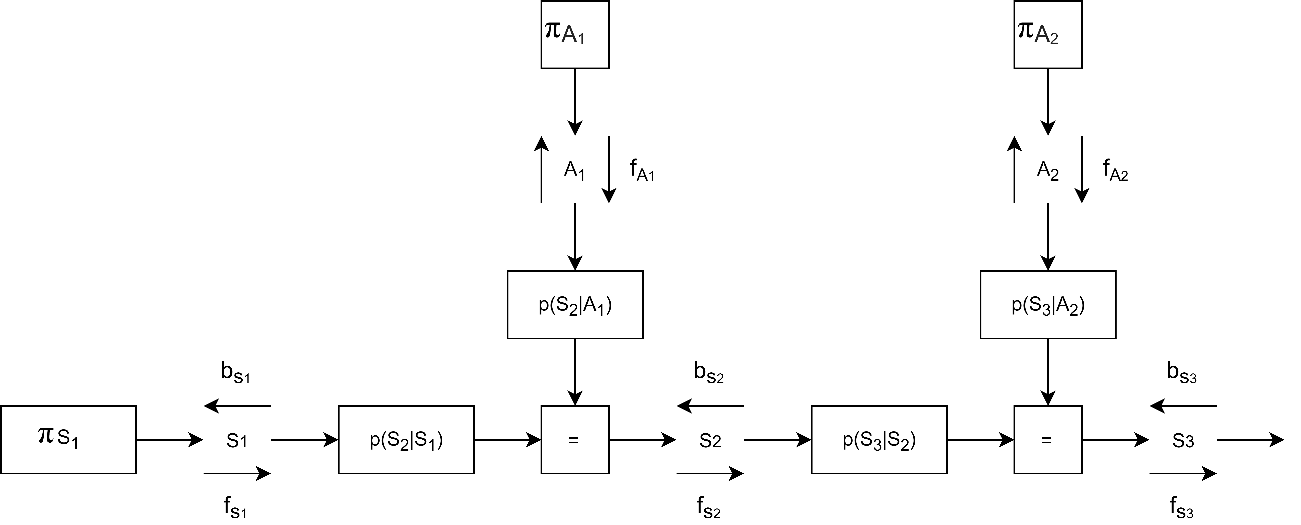
\includegraphics[width=10.5 cm]{res/FGnr.png}
	\caption{Factor graph in normal reduced form}
\end{figure}

\begin{equation}
	\begin{array}{l}
	f_{(S_tA_t)^1}(s_ta_t)=\sum_{s_{t-1}a_{t-1}} p(s_t a_t|s_{t-1} a_{t-1}) 
	f_{(S_{t-1}A_{t-1})^3}(s_{t-1}a_{t-1}) ;\\
	b_{(S_{t-1}A_{t-1})^3}(s_{t-1}a_{t-1})\propto \sum_{s_t a_t} p(s_t a_t|s_{t-1}a_{t-1}) b_{(S_tA_t)^1}(s_ta_t);\\
	 f_{(S_tA_t)^2}(s_ta_t)= c_t(s_ta_t);\\
	b_{(S_tA_t)^2}(s_ta_t) \propto b_{(S_tA_t)^3}(s_ta_t) f_{(S_tA_t)^1}(s_ta_t); \\
	b_{(S_tA_t)^1}(s_ta_t) \propto f_{(S_tA_t)^2}(s_ta_t) b_{(S_tA_t)^3}(s_ta_t) ;\\
	f_{(S_tA_t)^3}(s_ta_t) \propto f_{(S_tA_t)^1}(s_ta_t) f_{(S_tA_t)^2}(s_ta_t).
	\end{array}
	\label{eq:prop}
	\end{equation} 





\subsection{Input data}
\colorbox{yellow}{TODO}
The developed module takes as input several sets of data divided into:
\begin{itemize}
\item Data for the construction of the parameterized map: wave motion (significant height, direction, period, etc.), 
	weather conditions (temperature, wind at 10 meters, marine pressure, rain, etc.);
\item Mission data: mission objectives, Cobalt start and goal positions, drone release positions(Intermediate positions), 
	mission duration, etc.;
\end{itemize}

\subsection{Algorithm}
\colorbox{yellow}{TODO}



 

\subsection{Communication}
\colorbox{yellow}{TODO}
The communication between all the components of the DSS can comunicate through a MQTT broker.
MQTT or Message Queue Telemetry Transport is a featherlight and effective message protocol developed for the Internet of effects( IoT). 
It allows bias to change data in a publish- subscribe model, where data is published by a sender and entered by one or further subscribers. The protocol is grounded on a customer- garçon armature where guests can publish or subscribe to motifs on a garçon( also known as a broker). MQTT is ideal for IoT bias because it consumes minimum bandwidth and has low above, making it able for low- authority and resource- constrained bias. 
Its simplicity, scalability, and trustability have made it popular with inventors and has come a standard-issue protocol in the IoT assiduity.
An MQTT broker is a intermediary mecca that acts as a communication broker between MQTT guests. It's responsible for entering, storing, and ranking dispatches between guests. When an MQTT customer publishes a communication to a special content, the broker receives the communication and forwards it to all acceded guests that are interested in that content. also, when an MQTT customer subscribes to a content, the broker stores the subscription and forwards any dispatches published on that content to the acceded customer.

On the other phase, an MQTT customer is a device or operation that communicates with an MQTT broker. It can be either a publisher, subscriber, or both. When a customer publishes a communication to a special content, it sends the communication to the broker, which also on it to all acceded guests. When a customer subscribes to a content, it sends a subscription request to the broker, which stores the subscription and forwards any dispatches published on that content to the acceded customer.

In summary, the MQTT broker acts as an conciliator between MQTT guests, entering and ranking dispatches, while the MQTT guests are the bias or operations that give with the broker, publishing and assenting to dispatches. Together, the MQTT broker and guests form a publish- subscribe network, allowing effective and dependable message in IoT surroundings.


\section{Results}
\colorbox{yellow}{TODO}


\section{Conclusions}
\colorbox{yellow}{TODO}

Future developments:
\begin{itemize}
	\item WGS84 coordinates-based algorithm (and/or projection with UTM);
\end{itemize}


%%%%%%%%%%%%%%%%%%%%%%%%%%%%%%%%%%%%%%%%%%
\section{Results}

This section may be divided by subheadings. It should provide a concise and precise description of the experimental results, their interpretation as well as the experimental conclusions that can be drawn.
\subsection{Subsection}
\subsubsection{Subsubsection}

Bulleted lists look like this:
\begin{itemize}
\item	First bullet;
\item	Second bullet;
\item	Third bullet.
\end{itemize}

Numbered lists can be added as follows:
\begin{enumerate}
\item	First item; 
\item	Second item;
\item	Third item.
\end{enumerate}

The text continues here. 

\subsection{Figures, Tables and Schemes}

All figures and tables should be cited in the main text as Figure~\ref{fig1}, Table~\ref{tab1}, etc.

\begin{figure}[H]

\includegraphics[width=10.5 cm]{Definitions/logo-mdpi}
\caption{This is a figure. Schemes follow the same formatting. If there are multiple panels, they should be listed as: (\textbf{a}) Description of what is contained in the first panel. (\textbf{b}) Description of what is contained in the second panel. Figures should be placed in the main text near to the first time they are cited. A caption on a single line should be centered.\label{fig1}}
\end{figure}   
\unskip

\begin{table}[H] 
\caption{This is a table caption. Tables should be placed in the main text near to the first time they are~cited.\label{tab1}}
\newcolumntype{C}{>{\centering\arraybackslash}X}
\begin{tabularx}{\textwidth}{CCC}
\toprule
\textbf{Title 1}	& \textbf{Title 2}	& \textbf{Title 3}\\
\midrule
Entry 1		& Data			& Data\\
Entry 2		& Data			& Data \textsuperscript{1}\\
\bottomrule
\end{tabularx}
\noindent{\footnotesize{\textsuperscript{1} Tables may have a footer.}}
\end{table}

The text continues here (Figure~\ref{fig2} and Table~\ref{tab2}).

% Example of a figure that spans the whole page width. The same concept works for tables, too.
\begin{figure}[H]
\begin{adjustwidth}{-\extralength}{0cm}
\centering

\includegraphics[width=15.5cm]{Definitions/logo-mdpi}
\end{adjustwidth}
\caption{This is a wide figure.\label{fig2}}
\end{figure}  

\begin{table}[H]
\caption{This is a wide table.\label{tab2}}
	\begin{adjustwidth}{-\extralength}{0cm}
		\newcolumntype{C}{>{\centering\arraybackslash}X}
		\begin{tabularx}{\fulllength}{CCCC}
			\toprule
			\textbf{Title 1}	& \textbf{Title 2}	& \textbf{Title 3}     & \textbf{Title 4}\\
			\midrule
\multirow[m]{3}{*}{Entry 1 *}	& Data			& Data			& Data\\
			  	                   & Data			& Data			& Data\\
			             	      & Data			& Data			& Data\\
                   \midrule
\multirow[m]{3}{*}{Entry 2}    & Data			& Data			& Data\\
			  	                  & Data			& Data			& Data\\
			             	     & Data			& Data			& Data\\
                   \midrule
\multirow[m]{3}{*}{Entry 3}    & Data			& Data			& Data\\
			  	                 & Data			& Data			& Data\\
			             	    & Data			& Data			& Data\\
                  \midrule
\multirow[m]{3}{*}{Entry 4}   & Data			& Data			& Data\\
			  	                 & Data			& Data			& Data\\
			             	    & Data			& Data			& Data\\
			\bottomrule
		\end{tabularx}
	\end{adjustwidth}
	\noindent{\footnotesize{* Tables may have a footer.}}
\end{table}

%\begin{listing}[H]
%\caption{Title of the listing}
%\rule{\columnwidth}{1pt}
%\raggedright Text of the listing. In font size footnotesize, small, or normalsize. Preferred format: left aligned and single spaced. Preferred border format: top border line and bottom border line.
%\rule{\columnwidth}{1pt}
%\end{listing}

Text.

Text.

\subsection{Formatting of Mathematical Components}

This is the example 1 of equation:
\begin{linenomath}
\begin{equation}
a = 1,
\end{equation}
\end{linenomath}
the text following an equation need not be a new paragraph. Please punctuate equations as regular text.
%% If the documentclass option "submit" is chosen, please insert a blank line before and after any math environment (equation and eqnarray environments). This ensures correct linenumbering. The blank line should be removed when the documentclass option is changed to "accept" because the text following an equation should not be a new paragraph.

This is the example 2 of equation:
\begin{adjustwidth}{-\extralength}{0cm}
\begin{equation}
a = b + c + d + e + f + g + h + i + j + k + l + m + n + o + p + q + r + s + t + u + v + w + x + y + z
\end{equation}
\end{adjustwidth}

% Example of a page in landscape format (with table and table footnote).
%\startlandscape
%\begin{table}[H] %% Table in wide page
%\caption{This is a very wide table.\label{tab3}}
%	\begin{tabularx}{\textwidth}{CCCC}
%		\toprule
%		\textbf{Title 1}	& \textbf{Title 2}	& \textbf{Title 3}	& \textbf{Title 4}\\
%		\midrule
%		Entry 1		& Data			& Data			& This cell has some longer content that runs over two lines.\\
%		Entry 2		& Data			& Data			& Data\textsuperscript{1}\\
%		\bottomrule
%	\end{tabularx}
%	\begin{adjustwidth}{+\extralength}{0cm}
%		\noindent\footnotesize{\textsuperscript{1} This is a table footnote.}
%	\end{adjustwidth}
%\end{table}
%\finishlandscape


Please punctuate equations as regular text. Theorem-type environments (including propositions, lemmas, corollaries etc.) can be formatted as follows:
%% Example of a theorem:
\begin{Theorem}
Example text of a theorem.
\end{Theorem}

The text continues here. Proofs must be formatted as follows:

%% Example of a proof:
\begin{proof}[Proof of Theorem 1]
Text of the proof. Note that the phrase ``of Theorem 1'' is optional if it is clear which theorem is being referred to.
\end{proof}
The text continues here.

%%%%%%%%%%%%%%%%%%%%%%%%%%%%%%%%%%%%%%%%%%
\section{Discussion}

Authors should discuss the results and how they can be interpreted from the perspective of previous studies and of the working hypotheses. The findings and their implications should be discussed in the broadest context possible. Future research directions may also be highlighted.

%%%%%%%%%%%%%%%%%%%%%%%%%%%%%%%%%%%%%%%%%%
\section{Conclusions}

This section is not mandatory, but can be added to the manuscript if the discussion is unusually long or complex.

%%%%%%%%%%%%%%%%%%%%%%%%%%%%%%%%%%%%%%%%%%
\section{Patents}

This section is not mandatory, but may be added if there are patents resulting from the work reported in this manuscript.

%%%%%%%%%%%%%%%%%%%%%%%%%%%%%%%%%%%%%%%%%%
\vspace{6pt} 

%%%%%%%%%%%%%%%%%%%%%%%%%%%%%%%%%%%%%%%%%%
%% optional
%\supplementary{The following supporting information can be downloaded at:  \linksupplementary{s1}, Figure S1: title; Table S1: title; Video S1: title.}

% Only for the journal Methods and Protocols:
% If you wish to submit a video article, please do so with any other supplementary material.
% \supplementary{The following supporting information can be downloaded at: \linksupplementary{s1}, Figure S1: title; Table S1: title; Video S1: title. A supporting video article is available at doi: link.}

%%%%%%%%%%%%%%%%%%%%%%%%%%%%%%%%%%%%%%%%%%
\authorcontributions{For research articles with several authors, a short paragraph specifying their individual contributions must be provided. The following statements should be used ``Conceptualization, X.X. and Y.Y.; methodology, X.X.; software, X.X.; validation, X.X., Y.Y. and Z.Z.; formal analysis, X.X.; investigation, X.X.; resources, X.X.; data curation, X.X.; writing---original draft preparation, X.X.; writing---review and editing, X.X.; visualization, X.X.; supervision, X.X.; project administration, X.X.; funding acquisition, Y.Y. All authors have read and agreed to the published version of the manuscript.'', please turn to the  \href{http://img.mdpi.org/data/contributor-role-instruction.pdf}{CRediT taxonomy} for the term explanation. Authorship must be limited to those who have contributed substantially to the work~reported.}

\funding{Please add: ``This research received no external funding'' or ``This research was funded by NAME OF FUNDER grant number XXX.'' and  and ``The APC was funded by XXX''. Check carefully that the details given are accurate and use the standard spelling of funding agency names at \url{https://search.crossref.org/funding}, any errors may affect your future funding.}

\institutionalreview{In this section, you should add the Institutional Review Board Statement and approval number, if relevant to your study. You might choose to exclude this statement if the study did not require ethical approval. Please note that the Editorial Office might ask you for further information. Please add “The study was conducted in accordance with the Declaration of Helsinki, and approved by the Institutional Review Board (or Ethics Committee) of NAME OF INSTITUTE (protocol code XXX and date of approval).” for studies involving humans. OR “The animal study protocol was approved by the Institutional Review Board (or Ethics Committee) of NAME OF INSTITUTE (protocol code XXX and date of approval).” for studies involving animals. OR “Ethical review and approval were waived for this study due to REASON (please provide a detailed justification).” OR “Not applicable” for studies not involving humans or animals.}

\informedconsent{Any research article describing a study involving humans should contain this statement. Please add ``Informed consent was obtained from all subjects involved in the study.'' OR ``Patient consent was waived due to REASON (please provide a detailed justification).'' OR ``Not applicable'' for studies not involving humans. You might also choose to exclude this statement if the study did not involve humans.

Written informed consent for publication must be obtained from participating patients who can be identified (including by the patients themselves). Please state ``Written informed consent has been obtained from the patient(s) to publish this paper'' if applicable.}

\dataavailability{We encourage all authors of articles published in MDPI journals to share their research data. In this section, please provide details regarding where data supporting reported results can be found, including links to publicly archived datasets analyzed or generated during the study. Where no new data were created, or where data is unavailable due to privacy or ethical re-strictions, a statement is still required. Suggested Data Availability Statements are available in section “MDPI Research Data Policies” at \url{https://www.mdpi.com/ethics}.} 

\acknowledgments{In this section you can acknowledge any support given which is not covered by the author contribution or funding sections. This may include administrative and technical support, or donations in kind (e.g., materials used for experiments).}

\conflictsofinterest{Declare conflicts of interest or state ``The authors declare no conflict of interest.'' Authors must identify and declare any personal circumstances or interest that may be perceived as inappropriately influencing the representation or interpretation of reported research results. Any role of the funders in the design of the study; in the collection, analyses or interpretation of data; in the writing of the manuscript; or in the decision to publish the results must be declared in this section. If there is no role, please state ``The funders had no role in the design of the study; in the collection, analyses, or interpretation of data; in the writing of the manuscript; or in the decision to publish the~results''.} 

%%%%%%%%%%%%%%%%%%%%%%%%%%%%%%%%%%%%%%%%%%
%% Optional
\sampleavailability{Samples of the compounds ... are available from the authors.}

%% Only for journal Encyclopedia
%\entrylink{The Link to this entry published on the encyclopedia platform.}

\abbreviations{Abbreviations}{
The following abbreviations are used in this manuscript:\\

\noindent 
\begin{tabular}{@{}ll}
MDPI & Multidisciplinary Digital Publishing Institute\\
DOAJ & Directory of open access journals\\
TLA & Three letter acronym\\
LD & Linear dichroism
\end{tabular}
}

%%%%%%%%%%%%%%%%%%%%%%%%%%%%%%%%%%%%%%%%%%
%% Optional
\appendixtitles{no} % Leave argument "no" if all appendix headings stay EMPTY (then no dot is printed after "Appendix A"). If the appendix sections contain a heading then change the argument to "yes".
\appendixstart
\appendix
\section[\appendixname~\thesection]{}
\subsection[\appendixname~\thesubsection]{}
The appendix is an optional section that can contain details and data supplemental to the main text---for example, explanations of experimental details that would disrupt the flow of the main text but nonetheless remain crucial to understanding and reproducing the research shown; figures of replicates for experiments of which representative data are shown in the main text can be added here if brief, or as Supplementary Data. Mathematical proofs of results not central to the paper can be added as an appendix.

\begin{table}[H] 
\caption{This is a table caption.\label{tab5}}
\newcolumntype{C}{>{\centering\arraybackslash}X}
\begin{tabularx}{\textwidth}{CCC}
\toprule
\textbf{Title 1}	& \textbf{Title 2}	& \textbf{Title 3}\\
\midrule
Entry 1		& Data			& Data\\
Entry 2		& Data			& Data\\
\bottomrule
\end{tabularx}
\end{table}

\section[\appendixname~\thesection]{}
All appendix sections must be cited in the main text. In the appendices, Figures, Tables, etc. should be labeled, starting with ``A''---e.g., Figure A1, Figure A2, etc.

%%%%%%%%%%%%%%%%%%%%%%%%%%%%%%%%%%%%%%%%%%
\begin{adjustwidth}{-\extralength}{0cm}
%\printendnotes[custom] % Un-comment to print a list of endnotes

\reftitle{References}

% Please provide either the correct journal abbreviation (e.g. according to the “List of Title Word Abbreviations” http://www.issn.org/services/online-services/access-to-the-ltwa/) or the full name of the journal.
% Citations and References in Supplementary files are permitted provided that they also appear in the reference list here. 

%=====================================
% References, variant A: external bibliography
%=====================================
%\bibliography{your_external_BibTeX_file}

%=====================================
% References, variant B: internal bibliography
%=====================================
\begin{thebibliography}{10}
	\expandafter\ifx\csname url\endcsname\relax
	  \def\url#1{\texttt{#1}}\fi
	\expandafter\ifx\csname urlprefix\endcsname\relax\def\urlprefix{URL }\fi
	\expandafter\ifx\csname href\endcsname\relax
	  \def\href#1#2{#2} \def\path#1{#1}\fi
	
	\bibitem{CosciaFusion2018}
	P.~{Coscia}, F.~A. {N. Palmieri}, P.~{Braca}, L.~M. {Millefiori}, P.~{Willett},
	  Unsupervised maritime traffic graph learning with mean-reverting stochastic
	  processes, in: 2018 21st International Conference on Information Fusion
	  (FUSION), 2018, pp. 1822--1828.
	
	\bibitem{CosciaIEEE2018}
	P.~Coscia, P.~Braca, L.~M. Millefiori, F.~A.~N. Palmieri, P.~K. Willett,
	  Multiple ornstein-uhlenbeck processes for maritime traffic graph
	  representation, IEEE Transactions on Aerospace and Electronic Systems 54
	  (2018) 2158--2170.
	\newblock \href {https://doi.org/10.1109/TAES.2018.2808098}
	  {\path{doi:10.1109/TAES.2018.2808098}}.
	
	\bibitem{coscia2020}
	P.~Coscia, L.~Ballan, F.~Palmieri, A.~Alahi, S.~Savarese, Linear Artificial
	  Forces for Human Dynamics in Complex Contexts, Vol. 151, Springer Singapore,
	  2020, Ch.~2, pp. 21--33.
	\newblock \href {https://doi.org/doi.org/10.1007/978-981-13-8950-4\_3}
	  {\path{doi:doi.org/10.1007/978-981-13-8950-4\_3}}.
	
	\bibitem{CosciaIVC2018}
	P.~Coscia, F.~Castaldo, F.~A.~N. Palmieri, A.~Alahi, S.~Savarese, L.~Ballan,
	  Long-term path prediction in urban scenarios using circular distributions,
	  Image and Vision Computing 69 (2018) 81--91, (Editors Choice Award 2021).
	\newblock \href {https://doi.org/doi.org/10.1016/j.imavis.2017.11.006}
	  {\path{doi:doi.org/10.1016/j.imavis.2017.11.006}}.
	
	\bibitem{CosciaFusion2016}
	P.~Coscia, F.~Castaldo, F.~A.~N. Palmieri, L.~Ballan, A.~Alahi, S.~Savarese,
	  Point-based path prediction from polar histograms, in: Proceedings of the
	  19th International Conference on Information Fusion (FUSION 2016), 2016, pp.
	  1961--1967.
	
	\bibitem{CastaldoWirn2014}
	F.~Castaldo, F.~Palmieri, C.~Regazzoni, Application of Bayesian Techniques to
	  Behavior Analysis in Maritime Environments, Vol.~37, Springer, Cham, 2014,
	  Ch.~5, pp. 175--183.
	\newblock \href {https://doi.org/doi.org/10.1007/978-3-319-18164-6\_17}
	  {\path{doi:doi.org/10.1007/978-3-319-18164-6\_17}}.
	
	\bibitem{Loeliger2004}
	H.~A. Loeliger, An introduction to factor graphs, IEEE Signal Processing
	  Magazine 21~(1) (2004) 28 -- 41.
	
	\bibitem{Palmieri2016}
	F.~A.~N. Palmieri, A comparison of algorithms for learning hidden variables in
	  bayesian factor graphs in reduced normal form, IEEE Transactions on Neural
	  Networks and Learning Systems 27~(11) (2016) 2242--2255.
	
	\bibitem{Loeliger2007a}
	H.~A. Loeliger, J.~Dauwels, J.~Hu, S.~Korl, P.~Li, F.~Kschischang, The factor
	  graph approach to model-based signal processing, Proceedings of the IEEE
	  95~(6) (2007) 1295 --1322.
	
	\bibitem{DiGennaro2021}
	G.~Di~Gennaro, A.~Buonanno, F.~A.~N. Palmieri, Optimized realization of
	  bayesian networks in reduced normal form using latent variable model, Soft
	  Computing 25 (2021) 7029–7040.
	
	\bibitem{Buonanno2015b}
	A.~Buonanno, F.~A.~N. Palmieri, Two-dimensional multi-layer factor graphs in
	  reduced normal form, in: Proceedings of the International Joint Conference on
	  Neural Networks, IJCNN2015, July 12-17, 2015, Killarney, Ireland, 2015.
	
	\bibitem{Attias2003}
	H.~Attias, Planning by probabilistic inference, in: Proc. of the 9th Int.
	  Workshop on Artificial Intelligence and Statistics, 2003, p.~.
	
	\bibitem{bertsekas2019control}
	D.~P. Bertsekas, Reinforcement Learning and Optimal Control, Athena Scientific,
	  2019.
	
	\bibitem{Touissaint2006}
	M.~Toussaint, A.~Storkey, Probabilistic inference for solving discrete and
	  continuous state markov decision processes, Proceedings of the 23rd
	  International Conference on Machine Learning 2006 (2006) 945--952.
	\newblock \href {https://doi.org/10.1145/1143844.1143963}
	  {\path{doi:10.1145/1143844.1143963}}.
	
	\bibitem{Toussaint2009}
	M.~Toussaint, Probabilistic inference as a model of planned behavior,
	  Kunstliche Intelligenz 3 (01 2009).
	
	\bibitem{Todorov2009}
	E.~Todorov, Efficient computation of optimal actions, Proceedings of the
	  National Academy of Sciences 106~(28) (2009) 11478--11483.
	
	\bibitem{Kappen2013}
	H.~Kappen, V.~Gomez, M.~Opper, Optimal control as a graphical model inference
	  problem, in: Proceedings of the Twenty-Third International Conference on
	  Automated Planning and Scheduling, 2013.
	
	\bibitem{Ortega2013}
	P.~A. Ortega, D.~A. Braun, Thermodynamics as a theory of decision-making with
	  information-processing costs, Proceedings of the Royal Society A (May 2013).
	
	\bibitem{Levine2018}
	S.~Levine, Reinforcement learning and control as probabilistic inference:
	  Tutorial and review, arXiv:1805.00909v3 [cs.LG] 20 May 2018 (2018).
	
	\bibitem{Buckley2017}
	C.~L. Buckley, C.~S. Kim, S.~McGregor, A.~K. Seth, The free energy principle
	  for action and perception: a mathematica review, Journal of Mathematica
	  Phychology 81 (2017) 55--79.
	
	\bibitem{Parr2018}
	T.~Parr, K.~J. Friston, Generalised free energy and active inference: can the
	  future cause the past?, BioARXIV (2018).
	\newblock \href {https://doi.org/10.1101/304782} {\path{doi:10.1101/304782}}.
	
	\bibitem{Baltieri2017}
	M.~Baltieri, C.~L. Buckley, An active inference implementation of phototaxis,
	  ARXIV (2017).
	
	\bibitem{Zenon2018}
	Z.~Alexandre, S.~Oleg, P.~Giovanni, An information-theoretic perspective on the
	  costs of cognition, Neuropsychologia 123 (2018) 5--18.
	\newblock \href {https://doi.org/10.1016/j.neuropsychologia.2018.09.013}
	  {\path{doi:10.1016/j.neuropsychologia.2018.09.013}}.
	
	\bibitem{ParrFrontiers2018}
	T.~Parr, K.~J. Friston, The anatomy of inference: Generative models and brain
	  structure, Frontiers in Computational Neuroscience 12 (2018).
	\newblock \href {https://doi.org/10.3389/fncom.2018.00090}
	  {\path{doi:10.3389/fncom.2018.00090}}.
	
	\bibitem{Kaplan2018}
	R.~Kaplan, K.~J. Friston, Planning and navigation as active inference,
	  Biological Cybernetics 112 (2018) 323--347.
	\newblock \href {https://doi.org/10.1007/s00422-018-0753-2}
	  {\path{doi:10.1007/s00422-018-0753-2}}.
	
	\bibitem{NairSavareseetal2019}
	S.~Nair, Y.~Zhu, S.~Savarese, F.-F. Li, Causal induction from visual
	  observations for goal directed tasks, arXiv:1910.01751v1 [cs.LG] 3 Oct 2019
	  (2019).
	
	\bibitem{palmieri2021unified}
	F.~A.~N. Palmieri, K.~R. Pattipati, G.~D. Gennaro, G.~Fioretti, F.~Verolla,
	  A.~Buonanno, A unifying view of estimation and control using belief
	  propagation with application to path planning, IEEE Access 10 (2022)
	  15193--15216.
	\newblock \href {https://doi.org/10.1109/ACCESS.2022.3148127}
	  {\path{doi:10.1109/ACCESS.2022.3148127}}.
	
	\bibitem{palmieri2020path}
	F.~A.~N. Palmieri, K.~R. Pattipati, G.~Fioretti, G.~Di~Gennaro, A.~Buonanno,
	  {Path Planning Using Probability Tensor Flows}, IEEE Aerospace and Electronic
	  Systems Magazine 36~(1), preliminary version on arXiv:2003.02774. (Jan.
	  2021).
	
	\bibitem{gasparetto2015pathplanning}
	A.~Gasparetto, P.~Boscariol, A.~Lanzutti, R.~Vidoni, Path planning and
	  trajectory planning algorithms: A general overview, Mechanisms and Machine
	  Science 29 (2015) 3--27.
	\newblock \href {https://doi.org/10.1007/978-3-319-14705-5\_1}
	  {\path{doi:10.1007/978-3-319-14705-5\_1}}.
	
	\bibitem{micromouse2013law}
	G.~Law, Quantitative comparison of flood fill and modified flood fill
	  algorithms, International Journal of Computer Theory and Engineering (2013)
	  503--508\href {https://doi.org/10.7763/IJCTE.2013.V5.738}
	  {\path{doi:10.7763/IJCTE.2013.V5.738}}.
	
	\bibitem{maze2017Tjiharjadi}
	S.~Tjiharjadi, M.~Wijaya, E.~Setiawan, Optimization maze robot using a* and
	  flood fill algorithm, International Journal of Mechanical Engineering and
	  Robotics Research 6 (2017) 366--372.
	\newblock \href {https://doi.org/10.18178/ijmerr.6.5.366-372}
	  {\path{doi:10.18178/ijmerr.6.5.366-372}}.
	
	\bibitem{lozano1979planning}
	T.~Lozano-P\'{e}rez, M.~A. Wesley, An algorithm for planning collision-free
	  paths among polyhedral obstacles, Commun. ACM 22~(10) (1979) 560–570.
	\newblock \href {https://doi.org/10.1145/359156.359164}
	  {\path{doi:10.1145/359156.359164}}.
	
	\bibitem{lozano1983space}
	T.~Lozano-Perez, Spatial planning: A configuration space approach, IEEE
	  Transactions on Computers C-32~(2) (1983) 108--120.
	
	\bibitem{canny1987voronoi}
	J.~Canny, B.~Donald, Simplified voronoi diagrams, Tech. rep., Massachusetts
	  Institute of Technology, USA (1987).
	
	\bibitem{takahashi1989motion}
	O.~{Takahashi}, R.~J. {Schilling}, Motion planning in a plane using generalized
	  voronoi diagrams, IEEE Transactions on Robotics and Automation 5~(2) (1989)
	  143--150.
	
	\bibitem{abbadi2015path}
	A.~Abbadi, V.~Prenosil, Collided path replanning in dynamic environments using
	  rrt and cell decomposition algorithms, in: Modelling and Simulation for
	  Autonomous Systems, Vol. 9055, 2015, pp. 131--143.
	\newblock \href {https://doi.org/10.1007/978-3-319-22383-4\_9}
	  {\path{doi:10.1007/978-3-319-22383-4\_9}}.
	
	\bibitem{abbadi2015planning}
	A.~Abbadi, V.~Prenosil, Safe path planning using cell decomposition
	  approximation, in: International Conference on Distance Learning, Simulation
	  and Communication, 2015, pp. 8--14.
	
	\bibitem{potential1992hwang}
	Y.~K. {Hwang}, N.~{Ahuja}, A potential field approach to path planning, IEEE
	  Transactions on Robotics and Automation 8~(1) (1992) 23--32.
	
	\bibitem{potential2016sabudin}
	S.~elia nadira, R.~Omar, C.~K.~N. Hailma, Potential field methods and their
	  inherent approaches for path planning 11 (2016) 10801--10805.
	
	\bibitem{potential2020yao}
	Q.~{Yao}, Z.~{Zheng}, L.~{Qi}, H.~{Yuan}, X.~{Guo}, M.~{Zhao}, Z.~{Liu},
	  T.~{Yang}, Path planning method with improved artificial potential field—a
	  reinforcement learning perspective, IEEE Access 8 (2020) 135513--135523.
	
	\bibitem{amato1996planning}
	N.~M. {Amato}, Y.~{Wu}, A randomized roadmap method for path and manipulation
	  planning, in: Proceedings of IEEE International Conference on Robotics and
	  Automation, Vol.~1, 1996, pp. 113--120 vol.1.
	
	\bibitem{nissoux1999roadmaps}
	C.~{Nissoux}, T.~{Simeon}, J.~. {Laumond}, Visibility based probabilistic
	  roadmaps, in: Proceedings 1999 IEEE/RSJ International Conference on
	  Intelligent Robots and Systems. Human and Environment Friendly Robots with
	  High Intelligence and Emotional Quotients (Cat. No.99CH36289), Vol.~3, 1999,
	  pp. 1316--1321 vol.3.
	
	\bibitem{Lavalle98exploringrandom}
	S.~M. Lavalle, Rapidly-exploring random trees: A new tool for path planning,
	  The annual research report (1998).
	
	\bibitem{Hart68}
	P.~E. Hart, N.~J. Nilsson, B.~Raphael, A formal basis for the heuristic
	  determination of minimum cost paths, IEEE Transactions on Systems Science and
	  Cybernetics 4~(2) (1968) 100--107.
	\newblock \href {https://doi.org/10.1109/TSSC.1968.300136}
	  {\path{doi:10.1109/TSSC.1968.300136}}.
	
	\bibitem{Stentz93}
	A.~Stentz, Optimal and efficient path planning for unknown and dynamic
	  environments, INTERNATIONAL JOURNAL OF ROBOTICS AND AUTOMATION 10 (1993)
	  89--100.
	
	\bibitem{Koenig2005}
	S.~Koenig, M.~Likhachev, \href{https://doi.org/10.1109/TRO.2004.838026}{Fast
	  replanning for navigation in unknown terrain}, Trans. Rob. 21~(3) (2005)
	  354–363.
	\newblock \href {https://doi.org/10.1109/TRO.2004.838026}
	  {\path{doi:10.1109/TRO.2004.838026}}.
	\newline\urlprefix\url{https://doi.org/10.1109/TRO.2004.838026}
	
	\bibitem{Choset2005}
	H.~Choset, K.~Lynch, S.~Hutchinson, G.~Kantor, W.~Burgard, L.~Kavraki,
	  S.~Thrun, Principles of Robot Motion: Theory, Algorithms, and
	  Implementations, MIT Press, 2005.
	
	\bibitem{Everett2019}
	M.~Everett, J.~Miller, J.~How, Planning beyond the sensing horizon using a
	  learned context, 2019 IEEE/RSJ International Conference on Intelligent Robots
	  and Systems (IROS) (2019) 1064--1071.
	
	\bibitem{Niroui2017}
	F.~Niroui, B.~Sprenger, G.~Nejat, Robot exploration in unknown cluttered
	  environments when dealing with uncertainty, in: 2017 IEEE International
	  Symposium on Robotics and Intelligent Sensors (IRIS), 2017, pp. 224--229.
	\newblock \href {https://doi.org/10.1109/IRIS.2017.8250126}
	  {\path{doi:10.1109/IRIS.2017.8250126}}.
	
	\bibitem{Yamauchi1997}
	B.~Yamauchi, A frontier-based approach for autonomous exploration, in:
	  Proceedings of the 1997 IEEE International Symposium on Computational
	  Intelligence in Robotics and Automation, CIRA '97, IEEE Computer Society,
	  USA, 1997, p. 146.
	
	\bibitem{Naghizadeh2020}
	A.~Naghizadeh, S.~Berenjian, D.~J. Margolis, D.~N. Metaxas, Gnm: Gridcell
	  navigational model, Expert Systems with Applications 148 (2020) 113217.
	\newblock \href {https://doi.org/https://doi.org/10.1016/j.eswa.2020.113217}
	  {\path{doi:https://doi.org/10.1016/j.eswa.2020.113217}}.
	
	\bibitem{Zhu2011}
	Q.~Zhu, J.~Hu, W.~Cai, L.~Henschen, A new robot navigation algorithm for
	  dynamic unknown environments based on dynamic path re-computation and an
	  improved scout ant algorithm, Applied Soft Computing 11~(8) (2011)
	  4667--4676.
	\newblock \href {https://doi.org/https://doi.org/10.1016/j.asoc.2011.07.016}
	  {\path{doi:https://doi.org/10.1016/j.asoc.2011.07.016}}.
	
	\bibitem{Santos2020}
	V.~Santos, F.~E. Otero, C.~G. Johnson, F.~Osorio, C.~Toledo, Exploratory path
	  planning for mobile robots in dynamic environments with ant colony
	  optimization, in: Genetic and Evolutionary Computation Conference (GECCO
	  '20), ACM, 2020.
	\newblock \href {https://doi.org/https://doi.org/10.1145/3377930.3390219}
	  {\path{doi:https://doi.org/10.1145/3377930.3390219}}.
	
	\bibitem{PalmieriICRA2020}
	F.~A.~N. Palmieri, K.~R. Pattipati, G.~Fioretti, F.~Verolla, G.~Di~Gennaro,
	  A.~Buonanno, Exploration/exploitation in path planning using probability
	  propagation, in: Proceeding of the IEEE Intermational Conference on Robotics
	  and Automation (ICRA 2020), 2nd Workshop on Long-Term Human Motion Prediction
	  (LHMP), 2020.
	
	\bibitem{Buonanno2015a}
	A.~Buonanno, F.~Palmieri, Simulink implementation of belief propagation in
	  normal factor graphs, Smart Innovation, Systems and Technologies 37 (2015)
	  11--20.
	
	\bibitem{DiGennaro2022}
	G.~Di~Gennaro, A.~Buonanno, G.~Fioretti, F.~Verolla, K.~R. Pattipati, F.~A.~N.
	  Palmieri, Probabilistic inference and dynamic programming: A unified approach
	  to multi-agent autonomous coordination in complex and uncertain environments,
	  Frontiers in Physics 10 (2022).
	\newblock \href {https://doi.org/10.3389/fphy.2022.944157}
	  {\path{doi:10.3389/fphy.2022.944157}}.
	
	\end{thebibliography}
	


% If authors have biography, please use the format below
%\section*{Short Biography of Authors}
%\bio
%{\raisebox{-0.35cm}{\includegraphics[width=3.5cm,height=5.3cm,clip,keepaspectratio]{Definitions/author1.pdf}}}
%{\textbf{Firstname Lastname} Biography of first author}
%
%\bio
%{\raisebox{-0.35cm}{\includegraphics[width=3.5cm,height=5.3cm,clip,keepaspectratio]{Definitions/author2.jpg}}}
%{\textbf{Firstname Lastname} Biography of second author}

% For the MDPI journals use author-date citation, please follow the formatting guidelines on http://www.mdpi.com/authors/references
% To cite two works by the same author: \citeauthor{ref-journal-1a} (\citeyear{ref-journal-1a}, \citeyear{ref-journal-1b}). This produces: Whittaker (1967, 1975)
% To cite two works by the same author with specific pages: \citeauthor{ref-journal-3a} (\citeyear{ref-journal-3a}, p. 328; \citeyear{ref-journal-3b}, p.475). This produces: Wong (1999, p. 328; 2000, p. 475)

%%%%%%%%%%%%%%%%%%%%%%%%%%%%%%%%%%%%%%%%%%
%% for journal Sci
%\reviewreports{\\
%Reviewer 1 comments and authors’ response\\
%Reviewer 2 comments and authors’ response\\
%Reviewer 3 comments and authors’ response
%}
%%%%%%%%%%%%%%%%%%%%%%%%%%%%%%%%%%%%%%%%%%
\PublishersNote{}
\end{adjustwidth}
\end{document}

